\usetikzlibrary{trees,shadows}
\providecommand{\Energy}[1]{E_{#1}}
\providecommand{\EnergyCol}{\Energy{col}}
\providecommand{\bb}[1]{d^{#1}(t)}
\providecommand{\trackp}[1]{u#1}
\providecommand{\pEnergy}[1]{E_{#1}}
\newcommand{\scenegraphicalmodel}{
  \begin{scope}[grow cyclic, line width=1.2,
      variablenode/.style={circle,circular drop shadow,draw=red,fill=white,thick},
      bboxfactor/.style= {rectangle,inner sep=2,fill=green!50!black,thick,text=green!50!black},
      collfactor/.style= {rectangle,inner sep=2,fill=blue,thick,text=blue},
      trackfactor/.style={rectangle,inner sep=2,fill=red,thick,text=red},
      obs/.style={fill=gray!30,draw=black,text=gray!30},
      prevf/.style={draw=green!20,text=gray},
      prevobsv/.style={draw=gray!10,fill=gray!1,text=gray},
      prevv/.style={draw=red!20,text=gray}
    ]
    \path[use as bounding box,clip] (-2.6, -5.5) rectangle (6.1,0.5);
    \draw (-2.5,-2.65) rectangle +(0.5,0.3);
    \draw (-2.0,-2.35) -- ++(0.15, 0.15) -- ++(0, -0.6) -- (-2.0, -2.65);
    \path
    (0, 0)  node [variablenode] (x6) {6}
    ++(0, -1.5) node [variablenode] (x2) {2}
    ++(2.5, 0)  node [variablenode] (x5) {5}
    +(0, 1.5)  node [variablenode,obs] (u) {\tiny{1}}
    +(.2,0.9)  node {$\trackp{t}$}
    +(.5, -2)   node [variablenode] (x3) {3}
    +(2.3, -3.5)   node [variablenode] (x4) {4}
    +(2.5, 0)  node [variablenode] (x1) {1}
    ;

    % Factors between nodes 6 and 2
    \draw (x6) edge [bend right=40] node [bboxfactor] (f26) {\tiny{1}} (x2);
    \path (f26) +(-0.75,0) node [variablenode,obs] (d6) {\tiny{1}} 
    +(-.7,-.8)  node {$\bb{6}$};
    \draw (f26) edge (d6);
    \draw (x6) edge [bend left=40] node [trackfactor] (ft26) {\tiny{1}} (x2);
    \draw (ft26) edge [bend left=10] (u);
    \draw (x6) edge node [collfactor] {\tiny{1}} (x2);

    % Factors for node 2
    \path (x2) ++(0,-1.25) node [variablenode,obs] (d2) {\tiny{1}} 
    +(-.8,0)  node {$\bb{2}$};
    \draw (x2) edge node [bboxfactor] {\tiny{1}} (d2);

    % Factors between nodes 2 and 5
    \draw (x2) edge [bend right=35] node [bboxfactor] (f25) {\tiny{1}} (x5);
    \draw (x2) edge [bend left=35] node [trackfactor] (ft25) {\tiny{1}} (x5);
    \draw (x2) edge [] node [collfactor] {\tiny{1}} (x5);
    \draw (ft25) edge (u);
    \path (x5) ++(-1.25,-1.25) node [variablenode,obs] (d5) {\tiny{1}} 
    +(.8,0)  node {$\bb{5}$};
    \draw (f25) edge (d5);

    % Factors between nodes 5 and 1
    \draw (x5) edge [bend right=35] node [bboxfactor] (f51) {\tiny{1}} (x1);
    \draw (x5) edge [bend left=35] node [trackfactor] (ft51) {\tiny{1}} (x1);
    \draw (x5) edge [] node [collfactor] {\tiny{1}} (x1);
    \draw (ft51) edge [bend right=35] (u);
    \path (x1) ++(-1.25,-1.25) node [variablenode,obs] (d1) {\tiny{1}} 
    +(.8,0.2)  node {$\bb{1}$};
    \draw (f51) edge (d1);

    % Factors for node 3
    \path (x3) ++(0,-1.25) node [variablenode,obs] (d3) {\tiny{1}} 
    +(.8,0)  node {$\bb{3}$};
    \draw (x3) edge node [bboxfactor] {\tiny{1}} (d3);

    % Factors for node 4
    \path (x4) ++(0,1.25) node [variablenode,obs] (d4) {\tiny{1}} 
    +(.8,0)  node {$\bb{4}$};
    \draw (x4) edge node [bboxfactor] {\tiny{1}} (d4);

    % Legend
    \path (-1.75,-4.0) node (l1s) {} (-0, -4.0) node [anchor=west] (l1e) {$\EnergyBBox$};
    \draw (l1s) edge node [bboxfactor] {\tiny{1}} (l1e);
    \path (-1.75,-4.5) node (l2s) {} (0, -4.5) node [anchor=west] (l2e) {$\EnergyCol$};
    \draw (l2s) edge node [collfactor] {\tiny{1}} (l2e);
    \path (-1.75,-5.0) node (l3s) {} (0, -5.0) node [anchor=west] (l3e) {$\EnergyTrack$};
    \draw (l3s) edge node [trackfactor] {\tiny{1}} (l3e);

  \end{scope}
}
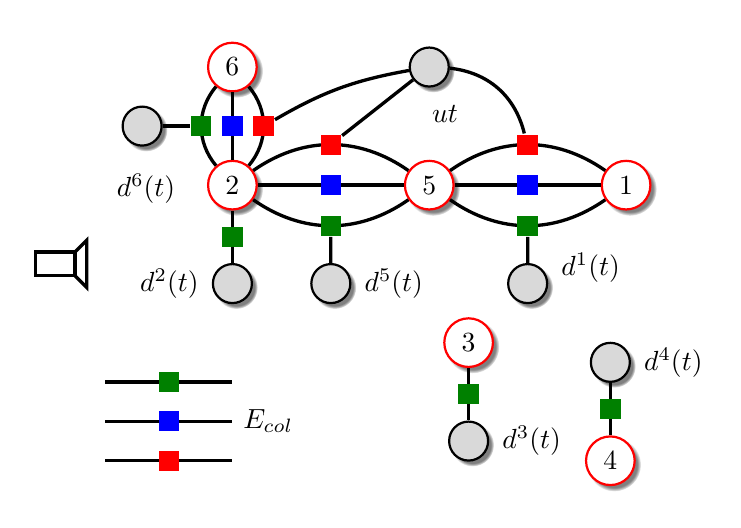
\begin{tikzpicture}
  \scenegraphicalmodel
\end{tikzpicture}
